\chapter{A note on imputing squares via polynomial combination approach}
\label{chap2}
	\begin{abstract}
		The polynomial combination (PC) method, proposed by Vink and Van Buuren, is a hot-deck multiple imputation method for imputation models containing squared terms. The method yields unbiased regression estimates and preserves the quadratic relationships in the imputed data for both MCAR and MAR mechanisms. However, Vink and Van Buuren never studied the coverage rate of the PC method. This paper investigates the coverage of the nominal 95\% confidence intervals for the polynomial combination method and improves the algorithm to avoid the perfect prediction issue. We also compare the original and the improved PC method to the substantive model compatible fully conditional specification method (SMC-FCS) proposed by Bartlett et al. and elucidate the two imputation methods' characters. 
	\end{abstract}

	\section{Introduction}
	Squared terms are often included in real-life data models to accommodate some form of nonlinearity. When the analysis model contains the partially observed covariates and corresponding squared terms, some challenges arise:  
	%such squared terms are part of an analysis model applied to incomplete data, 
	\begin{enumerate}
		\item The analysis and imputation models should accommodate squared terms, i.e., the squares themselves should be considered in the imputation procedure of corresponding linear terms.
		\item The relation between the square term and its lower-order polynomial should be preserved.
		\item The analysis model parameter estimates should be unbiased.
	\end{enumerate}
	
	To obtain unbiased estimates, one could impute the squared term as if it were another variable. We will refer to this as \textit{Transform, then Impute} (TTI) \citep{vonhippe2009}. However, this approach distorts the relationship between the original variable and its square. A straightforward process to preserve the quadratic relation during imputation is calculating the squared term only after imputation (\textit{Impute, then Transform}, ITT). However, ITT biases estimates of regression coefficients, as its contribution during imputation is ignored \citep{vonhippe2009, Vink2013}. Moreover, both these partial fixes only work when the missingness is completely random \citep{seaman2012multiple}.
	
	To solve these issues for a more general class of missingness mechanisms, \citet{Vink2013} propose to impute the combination of the original variable and its square and decompose it into distinct roots. This polynomial combination approach (PC) is built around predictive mean matching, a nonparametric imputation hot-deck technique that does not assume a specific distribution for the data \citep{rubin1986statistical, little1988missing}. \citet{seaman2012multiple} demonstrated that predictive mean matching gives biased estimation when the analysis is a linear regression with a quadratic term and the missingness mechanism is missing at random. However, PC yields unbiased estimates for MCAR and MAR missingness mechanisms by applying a reasonable donor selection procedure on the polynomial combination instead. 
	
	More recently, \citet{bartlett2015multiple} proposed a substantive model compatible approach (SMC-FCS), which generalizes the imputation of nonlinear covariates beyond the squared term model. The SMC-FCS technique is efficient but needs the correct data analysis model during imputation to obtain draws of values that conform to this model. It yields unbiased estimates if 1) the substantive model is correctly specified and 2) the normality assumption of missing variables with quadratic effects is tenable. When the missing variable with quadratic effects does not follow the normal distribution, one could apply an appropriate transformation to make the normality assumption plausible (e.g., log-normal distribution). More interestingly, \citet{bartlett2015multiple} suggest that the SMC-FCS estimates can yield unbiased inference, meaning that estimates are both unbiased and properly covered cf. \citet{neyman1934two}. Such an investigation into coverage of multiply imputed parameters was not part of the study by \citet{Vink2013}.
	
	We now have two techniques that seem promising in imputing squared terms: the polynomial combination method and SMC-FCS. Both approaches have appealing properties, preserve the relationship between the square and its base, and yield unbiased estimates. However, both techniques differ fundamentally in their approach. SMC-FCS is a strictly model-based technique that requires the correct specification of the complete-data model and the substantive model. On the other hand, PC is a hot-deck technique with a data-driven estimation procedure that only requires the specification of the polynomial combination. We highlighted the most used properties and promising methods in Table \ref{tab2_1} \citep{vonhippe2009, Vink2013, bartlett2015multiple}.
	\begin{table}[ht!]
		\resizebox{\textwidth}{!}{
			\begin{tabular}{c|c|c|c|c}
				& \texttt{TTI}           & \texttt{ITT}          & \texttt{PC}        & \texttt{SMC-FCS}      \\
				\hline
				Unbiased estimates of $\beta$          & MCAR only          & -            & MCAR \& MAR       & MCAR \& MAR          \\\hline
				Quadratic relationship & Not preserved & Preserved    & Preserved & Preserved    \\\hline
				Coverage rate of $\beta$         & Poor          & Poor         & Unknown   & Correct      \\\hline
				Violation of normality &     &    & Robust    & Somewhat robust   \\\hline
				Model specification    &   &  & Non-parametric  & Parametric
			\end{tabular}
		}
		\caption{Summary of properties of four squared term imputation methods.}
		\label{tab2_1}
	\end{table} 
	
	
	
	The interpretation of Table \ref{tab2_1}, taking the SMC-FCS approach as an example, should be as follows:
	\begin{enumerate}
		\item SMC-FCS yields unbiased regression estimates $\beta$ provided that the missing mechanism is \emph{MAR};
		\item SMC-FCS does \emph{preserve} the quadratic relationship between the original variable and its square;
		\item SMC-FCS produces \emph{correct} coverage rates of corresponding regression estimates $\beta$; 
		\item SMC-FCS is \emph{somewhat robust} against the violation of normality assumption of the covariates with quadratic effects;
		\item SMC-FCS is a \emph{parametric} imputation approach, which means SMC-FCS requires an explicit specified imputation model. 
	\end{enumerate}
	The `` - " sign in a cell indicates that the method cannot produce unbiased estimates. Whether the PC method has a correct coverage rate is not thoroughly studied and will be investigated in the following section. There are four blank cells left because the TTI and ITT methods cannot produce unbiased regression estimates or preserve the quadratic relationships; it is redundant to investigate the violation of normality and model specification for them.    
	
	In this manuscript, we evaluate the performance of imputing squared terms with SMC-FCS and the PC method to investigate these techniques' strengths and limitations in different scenarios. In the next section, we briefly discuss the SMC-FCS and PC methodology and propose a minor adjustment to the PC method.
	
	\section{Polynomial combination}
	In this paragraph we detail both the original polynomial combination (OPC) approach proposed by \citet{Vink2013}, as well as a modification that is robust against perfect prediction issues. We refer to the modified polynomial combination approach as MPC. 
	\subsection{Original polynomial combination}
	Suppose the model of scientific interest is 
	\begin{equation}
		Y = \alpha + X\beta_{1} + X^2\beta_{2} +\epsilon
		\label{eqn2_1}
	\end{equation}
	with $\epsilon \sim N(0, \sigma^2)$. We assume that $Y$ is complete and that $X = (X_{obs}, X_{mis})$ is partially missing. 
	
	The original polynomial combination method first performs predictive mean matching (PMM) \citep{little1988missing} on the combined variable $Z = X\beta_{1} + X^2\beta_{2}$, and then decomposes $Z$ into components $X$ and $X^2$. Under the model in equation \ref{eqn2_1}, two roots of variable $X$ are:
	\begin{equation}
		\begin{array}{ll}
			X_{-} &= -\frac{1}{2\beta_{2}}(\sqrt{4\beta_{2}Z + \beta_{1}^2} + \beta_{1})\\
			X_{+} &= \frac{1}{2\beta_{2}}(\sqrt{4\beta_{2}Z + \beta_{1}^2} - \beta_{1})
		\end{array}
	\end{equation} 
	where the discriminant $4\beta_{2}Z + \beta_{1}^2$ should be larger than 0. For any imputed $Z$, we select either $X = X_{-}$ or $X = X_{+}$ and square it to derive the square term $X^2$. 
	
	The choice between the roots $X_{-}$ and $X_{+}$is made by random sampling, conditional on $Y$, $Z$, and their interaction $YZ$. The binary random variable $V$ is defined as 0 if $X < X_{min}$ and 1 if $X > X_{min}$, where the minimum of the parabola $X_{min} = -\beta_{1}/2\beta_{2}$. We model the probability $P(V = 1)$ by logistic regression as
	\begin{equation}
		\textnormal{logit} P(V = 1) = Y\beta_{\textnormal{Y}} + Z\beta_{\textnormal{Z}} + YZ\beta_{\textnormal{YZ}}
	\end{equation} 
	on the observed data. Under the assumption of ignorability, we apply the same model to calculate the predicted probability $P(V = 1)$ for $X_{mis}$. Finally, a random draw from the binomial distribution is made ($P = 0$ \textnormal{or} $1$), and the corresponding (negative or positive) root is selected as the imputation for each missing value $X_{mis}$.  
	%See Vink and Van Buuren (2013) for computational details.  
	\subsection{Modification of Polynomial combination}
	Since we estimate binary variables $V$ in the OPC imputation procedure, it is necessary to avoid bias due to perfect prediction. When imputers apply the original polynomial combination method, perfect prediction occurs when all the observed binary variables $V_{obs}$ are equal to one (or zero). In this case, the likelihood tends to a limit as one or some regression coefficients tend to infinity, which leads to seriously implausible imputations of the binary variable $V$ \citep{white2010avoiding}. 
	
	Suppose all observed $X$ are located on the parabolic function's right arm, the perfect prediction arises. If no corrections are performed, the coefficients of the logistic function $\textnormal{logit}P(V = 1) = Y\beta_{Y} + Z\beta_{Z} + YZ\beta_{YZ}$ will have extremely wide and flat posterior distributions, which tends to derive extremely positive or negative estimates of coefficients. Provided all observed $X$ are located on the right arm of the parabolic function, some missing values of $X$ would be addressed incorrectly on the left arm, as shown in Figure 2.1(a).
	
	A computationally convenient approach to perfect prediction is data augmentation \citep[Section 3.6.2]{Buuren2018}. We augment the data with a few extra observations and add a small weight to these observations. Specifically, suppose the data has \emph{p} predictors and a \emph{k} levels outcome, for each predictor $X_{j}, j = 1, \dots, p$, we add two observations where $X_{j}$ equals either $\bar{x}_{j} - s_{j}$ or $\bar{x}_{j} + s_{j}$ for all levels of the response ($\bar{x}_{j}$ is the mean of $X_{j}$ and $s_{j}$ is the standard deviation of $X_{j}$). Other variables are fixed to their mean. Thus we add \emph{2k} observations for each predictor and in total \emph{2pk} observations to the data. A small weight \emph{w = (p + 1)/2pk} is assigned to each additional observation to restrict their impact on the imputation model identification. 
	
	\begin{table}[ht!]
		\centering
		\begin{tabular}{c|c|l|l}
			& V & Y                              & Z                              \\\hline
			1 & 1 & E($Y_{obs}$) + SD($Y_{obs}$) & E($Z_{obs}$)                  \\
			2 & 1 & E($Y_{obs}$) - SD($Y_{obs}$) & E($Z_{obs}$)                  \\
			3 & 0 & E($Y_{obs}$) + SD($Y_{obs}$) & E($Z_{obs}$)                  \\
			4 & 0 & E($Y_{obs}$) - SD($Y_{obs}$) & E($Z_{obs}$)                  \\
			5 & 1 & E($Y_{obs}$)                  & E($Z_{obs}$) + SD($Z_{obs}$) \\
			6 & 1 & E($Y_{obs}$)                  & E($Z_{obs}$) - SD($Z_{obs}$) \\
			7 & 0 & E($Y_{obs}$)                  & E($Z_{obs}$) + SD($Z_{obs}$) \\
			8 & 0 & E($Y_{obs}$)                  & E($Z_{obs}$) - SD($Z_{obs}$)
		\end{tabular}
		\caption{Augmented data}
		\label{tab2_2}
	\end{table}
	
	To improve the polynomial combination method, we impute $V_{mis}$ by logistic regression of V given Y, Z, and YZ with the augmented data instead of the observed data. More specifically, based on the observed $V$, $Y$ and $Z$, the augmented data adds eight subjects shown in Table \ref{tab2_2}, with the weight $3/8$, to the observed data. When the population estimation of the probability $P(V = 1)$ equals one (or zero), we expect the modified polynomial combination method would provide more plausible imputations, as shown in Figure 2.1(b).
	
	
	
	
	\subsection{SMC-FCS} 
	The substantive model compatible fully conditional specification (SMC-FCS) is a parametric imputation method proposed by \citet{bartlett2015multiple}. In general, the missing predictor is imputed based on other predictors. A rejection sampling (e.g., Metropolis-Hastings algorithm) is used where the acceptance ratio is generated based on the likelihood of the substantive model. Suppose $\phi$ is a vector containing the coefficients of the model $f(Y|X)$ and $\theta_{i}, j = 1, \dots, p$ is a vector containing the coefficients of the model $f(X_{i}|X_{-i})$, where $X_{-i}$ are all the other covariates excluding $X_{i}$. The parametric density function of the partially observed variable $X_{i}$ is proportional to $f(Y|X, \phi)f(X_{i}|X_{-i}, \theta_{i})$, rooted in the Bayesian rule:
	\begin{equation}
		\begin{array}{ll}
			f(X_{i}|X_{-i}, Y) &= \frac{f(X_{i}, X_{-i}, Y)}{f(Y, X_{-i})}\\
			&\propto f(Y|X_{i}, X_{-i})f(X_{i}|X_{-i}).
		\end{array} 
	\end{equation}
	Since the density generally does not follow a standard parametric family, the rejection sampling is necessary to draw coefficients from the posterior distributions of $\phi$ and $\theta_{i}$. With the assumption of independent priors $f(\phi)$ and $f(\theta_{i})$, the posterior distributions of $\phi$ and $\theta_{i}$ would be:
	\begin{equation}
		\begin{array}{ll}
			\phi &\sim f(Y|X_{i}, X_{-i}, \phi)f(\phi)\\
			\theta_{i} &\sim f(X_{i}|X_{-i}, \theta_{i})f(\theta_{i}).
		\end{array}
	\end{equation}
	The statistical property of this approach is that if the substantive model $f(Y|X)$ is correctly specified, the imputation model will be congenial to the analysis model \citep{meng1994multiple}. The lack of congeniality can sometimes produce implausible imputations that result in biased inferences in the downstream analysis \citep{robins2000inference}. 
	\section{Evaluation}
	We evaluated the average biases, the coverage of nominal 95\% confidence intervals, and the average width of corresponding confidence intervals of the regression weights $\beta_{1}$ and $\beta_{2}$. 
	\subsection{Simulation setup}
	The outcome $Y$ was simulated according to the scientific model:
	\begin{equation}
		Y = \alpha + X\beta_{1} + X^2\beta_{2} +\epsilon
	\end{equation}
	with $\alpha = 0$, $\beta_{1} = 1$, $\beta_{2} = 1$ and  $\epsilon \sim N(0, \sigma_{\epsilon}^2)$. The value of $\sigma_{\epsilon}$ varied according to different distributions of $X$ so that the coefficient of determination $R^2$ was always equal to 0.75. 
	
	The predictor $X$ was generated from a normal, a skew-normal, or a normal mixture distribution. The mean of $X$ was either 0 or 1, and the variance was 1 for all three distributions. The abscissa at the parabolic minimum was $X = -1/2$. Hence, when the location of $X$ was 0, there was a strong U-shaped association between $Y$ and $X$. If $X$ had location 2, the relationship between $Y$ and $X$ would be somewhat linear. For the skew-normal distribution, we set the slant parameter to be 6 when the mean of $X$ equaled 0 and -3 when the mean of $X$ equaled 2. For the normal mixture distribution, $X$ was drawn from $N(-0.875, 0.234)$ and $N(0.875, 0.234)$ with equal probability to have mean 0 and $N(1.125, 0.234)$ and $N(2.875, 0.234)$ with equal probability to have mean 2. 
	
	We generated a sample of size $n = 100$ and repeated 1000 simulations for each missingness scenario. For each simulation scenario, 30 percent missingness was induced jointly in $X$ and $X^2$ for five missingness mechanisms: MCAR, MARleft, MARmid, MARtail, and MARright. Specifically, MCAR denotes that the probability of $X$ being missing is the same for all cases. While with a left-tailed (MARleft), centered (MARmid), both tailed (MARtail) or right-tailed (MARright) missingness mechanism, a higher probability of $X$ being missing is assigned to the units with low, centered, extreme and high values of $Y$ respectively. All missingness was generated with the \textbf{ampute} function \citep{Schouten2018} from the package \texttt{MICE} \citep{Buuren2011} in \texttt{R} \citep{R2018}. The \textbf{mice.impute.quadratic} function in the package \texttt{MICE} was modified by including data augmentation.
	\subsection{Simulation results}
	We compared five approaches: TTI, ITT, OPC, MPC and SMC-FCS and focused on some exciting findings of OPC, MPC and SMC-FCS. The results of the TTI and ITT simulations reiterated the corresponding conclusions in Table \ref{tab2_1}. In general, TTI did not preserve the quadratic relation. Even it gave unbiased and confidence-valid estimates in some cases (e.g., with MCAR and standard normal distribution $X$). Furthermore, ITT had considerable bias under nearly all combinations of missingness mechanisms and distributions of $X$. 
	
	Table \ref{tab2_3} shows the average biases, the coverage of the nominal 95\% confidence intervals, and the average width of confidence intervals for $\beta_1$ and $\beta_2$ when $E(X)$ equals 0. The outcome $Y$ follows a U-shape. With MCAR, MARleft and MARmid and when $X$ is distributed as normal, skewed normal or a mixture of two normals, OPC and MPC gave unbiased estimates and correct CI coverage. The CI coverage of SMC-FCS was close to 95\%. However, with $X$ skew-normal distributed MCAR and MARmid, SMC-FCS was slightly biased. With MARtail and MARright, SMC-FCS outperformed OPC and MPC when $X$ followed a normal distribution or a normal mixture distribution. OPC and MPC had slight bias and somewhat reduced CI coverage (approximately 85\%) with $X$ distributed according to a normal, a skewed normal or a mixture of two normals. SMC-FCS was unbiased and had CI coverage close to 95\% with normal and mixture normal. However, with skewed normal $X$, SMC-FCS was somewhat biased and the CI had slightly lower than nominal coverage.
	
	Table \ref{tab2_4} demonstrates the mean biases of $\beta_{1}$ and $\beta_{2}$, the empirical coverage and the mean width of the corresponding 95\% CIs where $X$ is location 2 and scale 1. The observed values of $Y$ are almost on the right arm of the quadratic function. With normal $X$, SMC-FCS consistently yielded confidence-valid estimates because of the congeniality of the analysis model and imputation model. However, with MAR (MARleft, MARmid, MARtial and MARright), SMC-FCS gave a slight bias estimate for $\beta_{1}$. OPC and MPC gave unbiased results and the CI had approximately 95\% coverage with MCAR and MARmid. With MARleft, OPC and MPC were slightly biased for $\beta_{1}$, but the 95\% CI for $\beta_{1}$ and $\beta_{2}$ had the correct coverage. With MARtial and MARright, OPC and MPC were unbiased. The CI of MPC (around 90\%) had higher nominal coverage than OPC (around 80\%). With $X$ distributed according to a skewed normal, OPC and MPC yielded unbiased estimates with MCAR, MARmid, MARtail and MARright but slightly biased estimates with MARleft. The CI coverage of OPC and MPC was close to 95\% with MCAR, MARleft and MARmid. Like the case with normal $X$, the CI of MPC (around 90\%) had better coverage than OPC (around 85\%). With $X$ distributed as a mixture of two normals, SMC-FCS gave biased results under all missingness mechanisms and its CI had somewhat reduced coverage with MARright. OPC and MPC were unbiased with MCAR, MARmid and MARtail but biased with MARleft and MARright. MPC had CI coverage close to 95\% under all missingness mechanisms. The CI from OPC had correct coverage with MCAR, MARleft and MARmid, but approximately 85\% coverage with MARtail and MARright.         
	
	
	We investigated if the biases of SMC-FCS were caused by Monte Carlo error. Figures 2.2(a) and 2.2(b) demonstrate that the bias is somewhat systematic and not due to simulation error. The estimates for $\beta_{1}$ and $\beta_{2}$ show primarily overestimation and underestimation, respectively. This implies that, when applying SMC-FCS, the explicit specification of the distribution of the incomplete variable with the quadratic effect may need careful consideration.
	
	\section{Conclusion}
	We evaluated the performance of four imputation approaches for incomplete data problems where the model of scientific interest contains squared terms. We improved the performance of the polynomial combination method by incorporating a data augmentation step, thus realizing more plausible imputations when the missingness covariate relates almost exclusively to one arm of the quadratic curve.
	
	
	In our simulation studies, ITT gave biased estimates under almost all combinations of experimental factors, and TTI cannot preserve the quadratic relations in the imputed data. With normally distributed predictors and right-tailed missingness mechanisms, the performance of SMC-FCS was superior to that of MPC, with coverages closer to the nominal level. However, when the normality assumption is violated, the polynomial combination yields less biased estimates. Overall, both the SMC-FCS and polynomial combination methods produce plausible imputations of squared terms and outperform TTI and ITT. Differences between the approaches only become apparent under intense MARtail and MARright scenarios in simulation. However, these two mechanisms are more extreme than we are likely to see in practice since there is a strong relationship between the outcome $Y$ and the probability of the variable $X$ being unobserved in the tail. All in all, when differences in performance are found, such differences are small, and it may be challenging to interpret them as meaningful. This means that, in practice, the choice for an imputation approach could largely be a choice of preference. 
	
	If there is a solid, well-known scientific model, we highly recommend using SMC-FCS to sharpen results. The substantive model would then be correctly specified, ensuring that the distribution from which imputations are generated is compatible. SMC-FCS is a reliable model-based method to impute predictors with quadratic effects. It is theoretically well-grounded, and procedures are available for substantive models based on standard regression, discrete outcomes and proportional hazards \citep{Buuren2018}. However, with an increasing number of variables in the dataset, it becomes increasingly challenging to infer the correct substantive model based on the incomplete data a priori. The strategy of applying SMC-FCS in practice is performing model selection once imputed datasets are generated to ensure the accuracy of substantive model specification, which is not a trivial process \citep{bartlett2015multiple}. Usually, the substantive model is specified according to prior studies or assumptions.      
	
	In contrast, we advise using the polynomial combination approach when the scientific model is less specific or when modeling efforts are challenging. It is proven to be a valid data-driven imputation method that is flexible in applying because we only need to specify the quadratic term. This makes it straightforward to implement in any imputation effort. The polynomial combination method is based on predictive mean matching, and the performance of imputation procedures involving PMM are proven to work well in a wide range of research problems \citep{Vink2015, rubin1986statistical, little1988missing}. Therefore, we expect that the polynomial combination approach could be of great practical importance in incomplete data analyses with squared terms.  
	
	\newpage
	\begin{figure}[ht!]
		\begin{tabular}{c}
			\includegraphics[width=\textwidth, height=10cm]{plots/plot2.1.eps} \\
			\textnormal{(a)}  \\[6pt]
		\end{tabular}
		\begin{tabular}{c}
			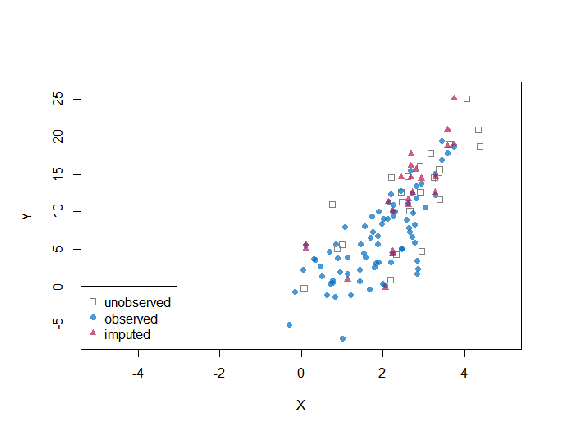
\includegraphics[width=\textwidth, height=10cm]{plots/plot2.2.eps}\\			
			\textnormal{(b)} \\[6pt]
		\end{tabular}
		\caption{Imputations (triangles) generated by OPC and MPC. We see that in (a) some imputations fall outside of the range of the observed (circle) and unobserved values (square), due to the OPC algorithm assigning the donor values to the incorrect distinct real root. In (b) the MPC approach assigns the imputations to the distinct real root that corresponds to the observed and unobserved data.}
		\label{fig2_1}
	\end{figure}
	
	
	\begin{figure}[ht!]
		\begin{tabular}{c}
			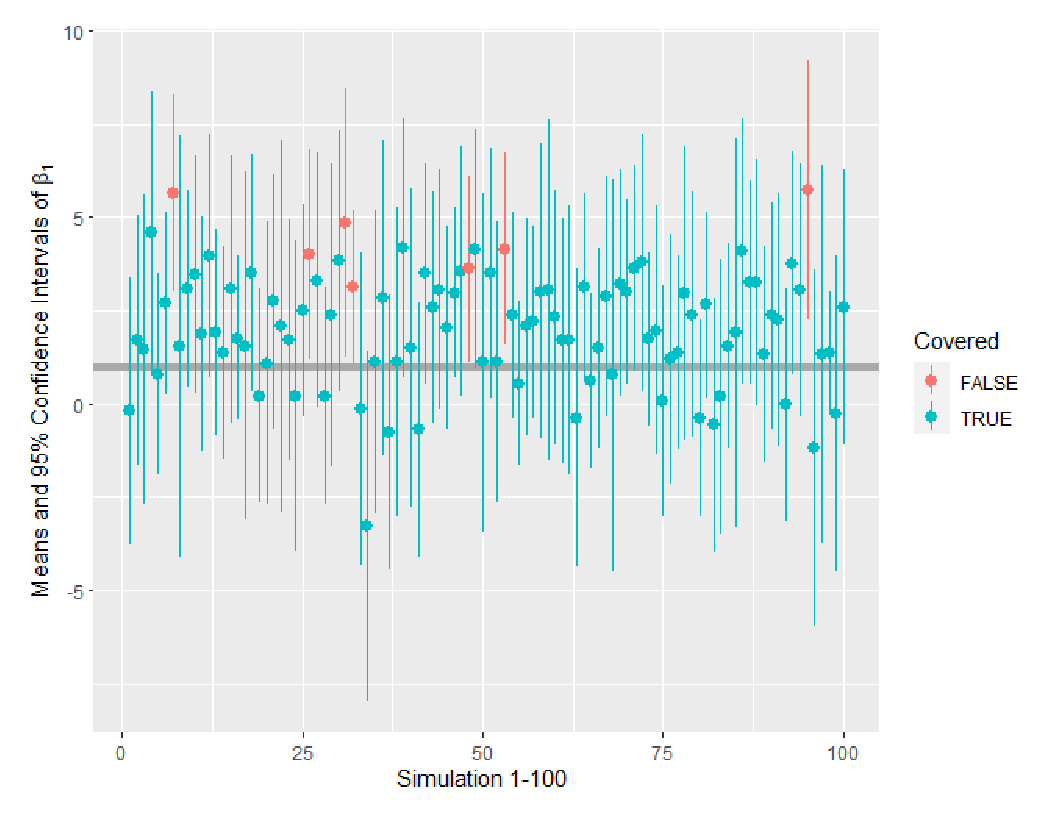
\includegraphics[width=\textwidth, height=10cm]{plots/plot2.3.eps} \\
			\textnormal{(a)}  \\[6pt]
		\end{tabular}
		\begin{tabular}{c}
			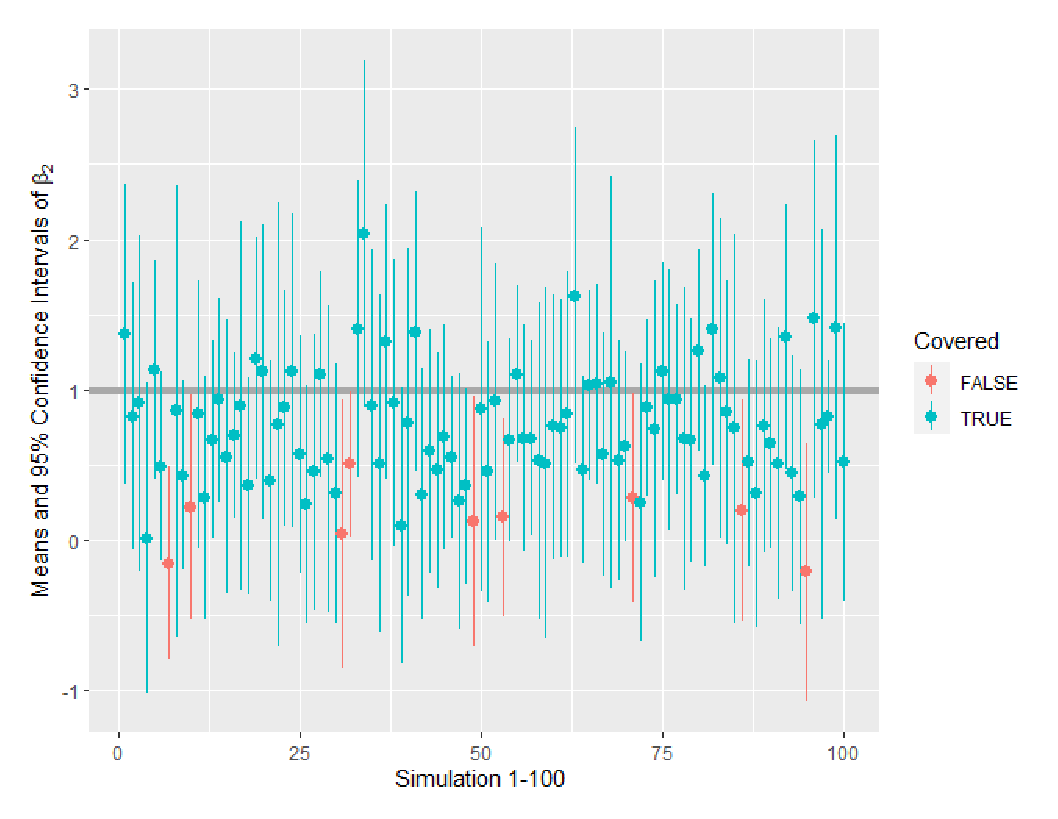
\includegraphics[width=\textwidth, height=10cm]{plots/plot2.4.eps}\\	
			\textnormal{(b)} \\[6pt]
		\end{tabular}
		\caption{The plot of means and confidence intervals of $\beta_{1}$ and $\beta_{2}$ from the first 100 simulations. The model of interest is $Y = X + X^2 + \epsilon$, where $X \sim \frac{1}{2}N(1.125, 0.234) + \frac{1}{2}N(2.875, 0.234)$. The missingness mechanism is MARright and the imputation approach is SMC-FCS. The imputations seem to primarily overestimate the true parameter estimate of $\beta_{1}$ in (a) and underestimate the true parameter estimate of $\beta_{2}$ in (b).}
		\label{fig2_2}
	\end{figure}
	

	\newpage
	\begin{table}[ht!]
		\resizebox{\textwidth}{!}{
			\begin{tabular}{c|ccc|ccc|ccc|ccc|ccc}
				& \multicolumn{15}{c}{Missingness Mechanism}                                                                                           \\
				& \multicolumn{3}{c}{MCAR} & \multicolumn{3}{c}{MARleft} & \multicolumn{3}{c}{MARmid} & \multicolumn{3}{c}{MARtail} & \multicolumn{3}{c}{MARright} \\
				& Bias    & Cov    & Ciw    & Bias    & Cov    & Ciw    & Bias    & Cov    & Ciw    & Bias    & Cov    & Ciw    & Bias   & Cov    & Ciw    \\
				\hline
				Normal         &        &        &        &        &        &        &        &        &        &        &        &        &        &        &        \\
				\texttt{TTI}            &        &        &        &        &        &        &        &        &        &        &        &        &        &        &        \\
				$\beta_1$      & 0.01  & 0.94  & 0.52  & -0.05  & 0.92  & 0.47  & -0.01  & 0.96   & 0.51  & 0.11  & 0.88  & 0.63  & 0.21  & 0.78  & 0.74  \\
				$\beta_2$      & 0  & 0.94  & 0.39  & -0.06  & 0.9  & 0.34  & -0.03  & 0.93  & 0.36  & 0.1  & 0.86  & 0.51  & 0.2  & 0.73  & 0.62  \\
				\texttt{ITT}            &        &        &        &        &        &        &        &        &        &        &        &        &        &        &        \\
				$\beta_1$      & -0.05  & 0.9  & 0.9  & -0.02  & 0.98  & 0.94  & -0.09  & 0.98   & 0.86  & -0.04  & 0.99  & 1.09  & -0.04  & 0.98  & 1.13  \\
				$\beta_2$      & -0.25  & 0.88  & 0.89  & -0.25  & 0.86  & 0.86  & -0.2  & 0.9  & 0.78  & -0.34  & 0.84  & 1.17  & -0.31  & 0.87  & 1.16  \\
				\texttt{OPC}            &        &        &        &        &        &        &        &        &        &        &        &        &        &        &        \\
				$\beta_1$      & 0.03  & 0.94  & 0.56  & 0.01  & 0.95  & 0.46  & 0.01  & 0.95   & 0.48  & 0.08  & 0.87  & 0.75  & 0.09  & 0.88  & 0.87  \\
				$\beta_2$      & 0.03  & 0.92  & 0.41  & 0  & 0.94  & 0.33  & 0  & 0.94  & 0.34  & 0.13  & 0.84  & 0.6  & 0.15  & 0.83  & 0.72  \\
				\texttt{MPC}            &        &        &        &        &        &        &        &        &        &        &        &        &        &        &        \\
				$\beta_1$      & 0.03  & 0.94  & 0.56  & 0.01  & 0.95  & 0.46  & 0.01      & 0.95  & 0.47  & 0.1  & 0.86  & 0.75  & 0.1  & 0.88  & 0.86  \\
				$\beta_2$      & 0.03  & 0.92  & 0.41  & 0  & 0.94  & 0.33  & 0  & 0.94  & 0.34  & 0.13   & 0.84  & 0.6  & 0.15  & 0.83  & 0.72  \\
				\texttt{SMC-FCS}        &        &        &        &        &        &        &        &        &        &        &        &        &        &        &        \\
				$\beta_1$      & 0  & 0.96  & 0.53  & -0.01  & 0.95  & 0.47  & 0.01  & 0.94  & 0.49  & 0  & 0.96  & 0.6  & 0  & 0.95  & 0.67  \\
				$\beta_2$      & 0  & 0.95  & 0.39  & 0  & 0.95  & 0.33  & 0  & 0.95  & 0.34  & 0.01  & 0.95  & 0.51  & 0.02  & 0.95  & 0.57  \\
				\hline
				Skewed-normal    &        &        &        &        &        &        &        &        &        &        &        &        &        &        &        \\
				\texttt{TTI}            &        &        &        &        &        &        &        &        &        &        &        &        &        &        &        \\
				$\beta_1$      & -0.15  & 0.95  & 3.21  & -0.25  & 0.92  & 2.98  & 0.15  & 0.95   & 2.79  & -0.43  & 0.92  & 4.93  & -0.26  & 0.94  & 5.75  \\
				$\beta_2$      & 0.09  & 0.94  & 1.48  & 0.04  & 0.93  & 1.28  & -0.09  & 0.94  & 1.23  & 0.35  & 0.88  & 2.59  & 0.39  & 0.91  & 3.28  \\
				\texttt{ITT}            &        &        &        &        &        &        &        &        &        &        &        &        &        &        &        \\
				$\beta_1$      & 0.3  & 0.94  & 2.55  & 0.27  & 0.93  & 2.24  & 0.18  & 0.96   & 2.39  & 0.5  & 0.9  & 2.91  & 0.41  & 0.94  & 3.18  \\
				$\beta_2$      & -0.13  & 0.96  & 1.27  & -0.12  & 0.93  & 1.01  & -0.07  & 0.96  & 1.07  & -0.24  & 0.9  & 1.71  & -0.15  & 0.95  & 1.91  \\
				\texttt{OPC}            &        &        &        &        &        &        &        &        &        &        &        &        &        &        &        \\
				$\beta_1$      & 0  & 0.93  & 2.68  & -0.02  & 0.94   & 2.49  & 0.03  & 0.93  & 2.4  & -0.07  & 0.86  & 3.64  & 0.01  & 0.82  & 3.79   \\
				$\beta_2$      & 0.03  & 0.92  & 1.27  & 0.01  & 0.94  & 1.11  & -0.01  & 0.94  & 1.08  & 0.16  & 0.85  & 1.98  & 0.13  & 0.82  & 2.16   \\
				\texttt{MPC}            &        &        &        &        &        &        &        &        &        &        &        &        &        &        &        \\
				$\beta_1$      & 0.01  & 0.95  & 2.69  & -0.02  & 0.94  & 2.47  & 0.03  & 0.93  & 2.39  & -0.02  & 0.92  & 3.87  & 0.03  & 0.88  & 4  \\
				$\beta_2$      & 0.03  & 0.94  & 1.29  & 0.01  & 0.94  & 1.11  & -0.01   & 0.93  & 1.08  & 0.15  & 0.91  & 2.09  & 0.15  & 0.86  & 2.26  \\
				\texttt{SMC-FCS}        &        &        &        &        &        &        &        &        &        &        &        &        &        &        &        \\
				$\beta_1$      & -0.14  & 0.94  & 2.59  & -0.01  & 0.95  & 2.39  & -0.15  & 0.96  & 2.43  & -0.41   & 0.93  & 3.51  & -0.49  & 0.91  & 3.56  \\
				$\beta_2$      & 0.09  & 0.95  & 1.21  & 0  & 0.94  & 1.08  & 0.07  & 0.96  & 1.07  & 0.28  & 0.91  & 1.87  & 0.39  & 0.88  & 1.97  \\
				\hline
				Normal-mixture &        &        &        &        &        &        &        &        &        &        &        &        &        &        &        \\
				\texttt{TTI}            &        &        &        &        &        &        &        &        &        &        &        &        &        &        &        \\
				$\beta_1$      & 0  & 0.96  & 0.4  & -0.05  & 0.93  & 0.38  & 0  & 0.95   & 0.4  & 0.02  & 0.95  & 0.43  & 0.1  & 0.86  & 0.46  \\
				$\beta_2$      & 0  & 0.96  & 0.46  & -0.05  & 0.94  & 0.42  & -0.04  & 0.95  & 0.44  & 0.02  & 0.96  & 0.52  & 0.09  & 0.91  & 0.57  \\
				\texttt{ITT}            &        &        &        &        &        &        &        &        &        &        &        &        &        &        &        \\
				$\beta_1$      & -0.04  & 0.98  & 0.62  & 0.03  & 0.98  & 0.59  & -0.02  & 0.98   & 0.58  & -0.07  & 0.98  & 0.65  & -0.09  & 0.98  & 0.68  \\
				$\beta_2$      & -0.42  & 0.59  & 0.98  & -0.36  & 0.71  & 0.96  & -0.32  & 0.72  & 0.86  & -0.55  & 0.35  & 0.97  & -0.52  & 0.4  & 0.96  \\ 
				\texttt{OPC}            &        &        &        &        &        &        &        &        &        &        &        &        &        &        &        \\
				$\beta_1$      & 0.02   & 0.94   & 0.38  & 0  & 0.93  & 0.36  & 0.01  & 0.94  & 0.37  & 0.06  & 0.88  & 0.44  & 0.08  & 0.87  & 0.48  \\
				$\beta_2$      & 0.01  & 0.94  & 0.44  & 0      & 0.93  & 0.41    & 0  & 0.94  & 0.41  & 0.04  & 0.92  & 0.53  & 0.05  & 0.92  & 0.58  \\
				\texttt{MPC}            &        &        &        &        &        &        &        &        &        &        &        &        &        &        &        \\
				$\beta_1$      & 0.02  & 0.94   & 0.38  & 0  & 0.93  & 0.36  & 0.01  & 0.94  & 0.36  & 0.06  & 0.89  & 0.44  & 0.08  & 0.87  & 0.48  \\
				$\beta_2$      & 0.01  & 0.95  & 0.44  & 0  & 0.94  & 0.41  & 0  & 0.94  & 0.4  & 0.04  & 0.92  & 0.53  & 0.05  & 0.93  & 0.58  \\
				\texttt{SMC-FCS}        &        &        &        &        &        &        &        &        &        &        &        &        &        &        &        \\
				$\beta_1$      & -0.01  & 0.95  & 0.4  & -0.02  & 0.95  & 0.38  & 0.02  & 0.95  & 0.38  & -0.05  & 0.93  & 0.43  & -0.05  & 0.93  & 0.48  \\
				$\beta_2$      & -0.02  & 0.95  & 0.46   & 0.01  & 0.94  & 0.41   & -0.03  & 0.94  & 0.42  & -0.03  & 0.94  & 0.51  & -0.06  & 0.93  & 0.57 
			\end{tabular}
		}
		\caption{Simulation results for five missingness mechanisms when imputing a squared term regression where the mean of X equals 0. Shown are absolute bias of the estimate, coverage of the 95\% confidence interval for the estimate and the average confidence interval width.}
		\label{tab2_3}
	\end{table}
	
	\newpage
	\begin{table}[ht!]
		\resizebox{\textwidth}{!}{
			\begin{tabular}{c|ccc|ccc|ccc|ccc|ccc}
				& \multicolumn{15}{c}{Missingness Mechanism}                                                                                               \\
				& \multicolumn{3}{c}{MCAR} & \multicolumn{3}{c}{MARleft} & \multicolumn{3}{c}{MARmid} & \multicolumn{3}{c}{MARtail} & \multicolumn{3}{c}{MARright} \\
				& Bias     & Cov    & Ciw    & Bias     & Cov    & Ciw    & Bias     & Cov    & Ciw    & Bias     & Cov    & Ciw    & Bias    & Cov    & Ciw    \\ \hline
				Normal                            &         &        &        &         &        &        &         &        &        &         &        &        &         &        &        \\
				\texttt{TTI}            &        &        &        &        &        &        &        &        &        &        &        &        &        &        &        \\
				$\beta_1$      & -0.58  & 0.93  & 7.17  & -1  & 0.92  & 8  & -0.08  & 0.95   & 6.04  & -1.32  & 0.91  & 10.11  & -0.89  & 0.93  & 9.24  \\
				$\beta_2$      & 0.11  & 0.93  & 1.66  & 0.15  & 0.93  & 1.73  & 0  & 0.95  & 1.39  & 0.31  & 0.89  & 2.43  & 0.29  & 0.91  & 2.4  \\
				\texttt{ITT}            &        &        &        &        &        &        &        &        &        &        &        &        &        &        &        \\
				$\beta_1$      & 0.71  & 0.94  & 5.61  & 0.6  & 0.94  & 5.57  & 0.5  & 0.96   & 5.27  & 0.99  & 0.92  & 5.95  & 1.02  & 0.93  & 4.97  \\
				$\beta_2$      & -0.19  & 0.95  & 1.41  & -0.14  & 0.95  & 1.31  & -0.13  & 0.96  & 1.28  & -0.28  & 0.9  & 1.58  & -0.3  & 0.91  & 1.63  \\
				\texttt{OPC}     &         &        &        &         &        &        &         &        &        &         &        &        &         &        &        \\
				$\beta_1$                         & -0.05  & 0.92  & 5.28  & -0.15   & 0.93  & 5.56  & 0.01   & 0.93  & 4.98  & -0.12   & 0.87  & 6.04  & 0.04   & 0.8  & 5.65  \\
				$\beta_2$                         & 0.02    & 0.93  & 1.27  & 0.03   & 0.94  & 1.27  & 0   & 0.94  & 1.17  & 0.05   & 0.87  & 1.51  & 0.03   & 0.82  & 1.48  \\
				\texttt{MPC}     &         &        &        &         &        &        &         &        &        &         &        &        &         &        &        \\
				$\beta_1$                         & -0.05   & 0.93  & 5.17  & -0.15   & 0.94  & 5.39  & 0   & 0.91  & 4.77  & -0.03   & 0.93  & 6.26  & 0.05   & 0.89  & 6.02  \\
				$\beta_2$                         & 0.02   & 0.93  & 1.25  & 0.03   & 0.94  & 1.24  & 0.01   & 0.92  & 1.13  & 0.04   & 0.91  & 1.56  & 0.04   & 0.88  & 1.57  \\
				\texttt{SMC-FCS} &         &        &        &         &        &        &         &        &        &         &        &        &         &        &        \\
				$\beta_1$                         & 0.03    & 0.95   & 5.44  & -0.11   & 0.95  & 5.78   & -0.06   & 0.95  & 5.14  & -0.22   & 0.94  & 6.02  & -0.1   & 0.97  & 5.69  \\
				$\beta_2$                         & 0   & 0.95  & 1.3  & 0.03   & 0.94  & 1.31  & 0.01   & 0.95  & 1.25  & 0.06    & 0.94  & 1.5  & 0.04   & 0.96  & 1.48  \\ \hline
				Skewed-normal                       &         &        &        &         &        &        &         &        &        &         &        &        &         &        &        \\
				\texttt{TTI}            &        &        &        &        &        &        &        &        &        &        &        &        &        &        &        \\
				$\beta_1$      & -0.15  & 0.93  & 2.95  & -0.45  & 0.92  & 4.14  & -0.06  & 0.95   & 2.56  & -0.32  & 0.95  & 4.07  & -0.07  & 0.94  & 2.97  \\
				$\beta_2$      & 0.06  & 0.93  & 1.27  & 0.14  & 0.92  & 1.59  & 0.03  & 0.95  & 1.11  & 0.12  & 0.94  & 1.73  & 0.06  & 0.93  & 1.41  \\
				\texttt{ITT}            &        &        &        &        &        &        &        &        &        &        &        &        &        &        &        \\
				$\beta_1$      & 0.46  & 0.92  & 2.64  & 0.29  & 0.93  & 2.86  & 0.35  & 0.94   & 2.49  & 0.62  & 0.87  & 2.83  & 0.73  & 0.81  & 2.48  \\
				$\beta_2$      & -0.28  & 0.88  & 1.26  & -0.13  & 0.94  & 1.23  & -0.21  & 0.9  & 1.16  & -0.37  & 0.8  & 1.37  & -0.48  & 0.64  & 1.26  \\
				\texttt{OPC}     &         &        &        &         &        &        &         &        &        &         &        &        &         &        &        \\
				$\beta_1$                         & 0.01   & 0.92  & 2.24  & -0.11   & 0.93  & 2.74   & 0.02   & 0.93  & 2.19  & -0.07   & 0.88  & 2.5  & 0   & 0.85  & 2.19  \\
				$\beta_2$                         & 0   & 0.93  & 0.99  & 0.05    & 0.93  & 1.14  & -0.01   & 0.94  & 0.96  & 0.04    & 0.89  & 1.11  & 0.02   & 0.86  & 1.03  \\
				\texttt{MPC}     &         &        &        &         &        &        &         &        &        &         &        &        &         &        &        \\
				$\beta_1$                         & 0   & 0.92  & 2.18  & -0.11   & 0.93  & 2.66  & 0   & 0.92  & 2.02  & -0.04    & 0.94  & 2.59  & 0.02   & 0.91  & 2.28  \\
				$\beta_2$                         & 0.01   & 0.93   & 0.96  & 0.05   & 0.93  & 1.11  & 0   & 0.93  & 0.89  & 0.04   & 0.95  & 1.15  & 0.02   & 0.9   & 1.06  \\
				\texttt{SMC-FCS} &         &        &        &         &        &        &         &        &        &         &        &        &         &        &        \\
				$\beta_1$                         & 0.1   & 0.95  & 2.46  & -0.04   & 0.95  & 3.01  & 0.09    & 0.95  & 2.27  & 0.14   & 0.95  & 2.65  & 0.2     & 0.93  & 2.22  \\
				$\beta_2$                         & -0.05   & 0.94  & 1.08  & 0.03  & 0.95  & 1.22  & -0.04   & 0.94  & 1  & -0.08   & 0.94  & 1.2    & -0.14   & 0.91  & 1.04  \\ \hline
				Normal-mixture                    &         &        &        &         &        &        &         &        &        &         &        &        &         &        &        \\
				\texttt{TTI}            &        &        &        &        &        &        &        &        &        &        &        &        &        &        &        \\
				$\beta_1$      & -1.5  & 0.9  & 10.48  & -2.15  & 0.86  & 11.93  & -0.71  & 0.93   & 8.8  & -2.35  & 0.87  & 13.63  & -1.73  & 0.91  & 12.47  \\
				$\beta_2$      & 0.33  & 0.9  & 2.52  & 0.43  & 0.87  & 2.73  & 0.16  & 0.94  & 2.11  & 0.51  & 0.88  & 3.29  & 0.43  & 0.9  & 3.15  \\
				\texttt{ITT}            &        &        &        &        &        &        &        &        &        &        &        &        &        &        &        \\
				$\beta_1$      & 1.38  & 0.88  & 6.4  & 0.83  & 0.92  & 6.13  & 1.07  & 0.92   & 6.33  & 1.76  & 0.8  & 6.08  & 2.08  & 0.78  & 6.35  \\
				$\beta_2$      & -0.35  & 0.88  & 1.62  & -0.19  & 0.94  & 1.52  & -0.25  & 0.92  & 1.58  & -0.49  & 0.76  & 1.57  & -0.57  & 0.72  & 1.63  \\	
				\texttt{OPC}     &         &        &        &         &        &        &         &        &        &         &        &        &         &        &        \\
				$\beta_1$                         & -0.05  & 0.92  & 6.28  & -0.24   & 0.92  & 6.51  & 0.02   & 0.93  & 6.05  & -0.09   & 0.88  & 6.61  & 0.19    & 0.85  & 6.43  \\
				$\beta_2$                         & 0.02    & 0.92   & 1.53  & 0.06   & 0.92  & 1.57  & 0   & 0.94  & 1.47   & 0.04   & 0.87  & 1.64  & -0.03   & 0.86  & 1.62  \\
				\texttt{MPC}     &         &        &        &         &        &        &         &        &        &         &        &        &         &        &        \\
				$\beta_1$                         & -0.04   & 0.93  & 6.24  & -0.23   & 0.92   & 6.39  & 0.02  & 0.91  & 5.92  & -0.04  & 0.93  & 6.77  & 0.24   & 0.92  & 6.69   \\
				$\beta_2$                         & 0.02   & 0.93  & 1.53  & 0.05    & 0.93  & 1.54  & 0   & 0.92   & 1.45  & 0.03   & 0.92   & 1.68  & -0.03   & 0.92   & 1.69  \\
				\texttt{SMC-FCS} &         &        &        &         &        &        &         &        &        &         &        &        &         &        &        \\
				$\beta_1$                         & 0.32   & 0.95  & 6.37  &-0.32   & 0.96  & 6.85   & 0.25   & 0.94  & 6.18  & 0.5   & 0.94  & 6.58  & 0.95   & 0.91  & 6.69  \\
				$\beta_2$                         & -0.07   & 0.94  & 1.57  & 0.09   & 0.95   & 1.65  & -0.04   & 0.94  & 1.5  & -0.14   & 0.92   & 1.66  & -0.25   & 0.9  & 1.71 
			\end{tabular}
		}
		\caption{Simulation results for five missingness mechanisms when imputing a squared term regression where the mean of X equals 2. Shown are absolute bias of the estimate, coverage of the 95\% confidence interval for the estimate and the average confidence interval width.}
		\label{tab2_4}
	\end{table}


